\fancyhead[R]{\slshape PHỤ LỤC}
\begin{center}
	\begin{huge}
			\textbf{PHỤ LỤC 1}\\
			\textit{Biểu diễn số thực dạng nhị phân}
	\end{huge}
\end{center}

Có bốn đinh dạng chuẩn IEEE biểu diễn số dấu chấm động ở dạng phị phân được sử dụng trong bộ xử lý Intel:
\begin{longtable}{|l|m{2cm}|m{3cm}|m{3cm}|l|l|}
	\hline
		Kiểu & Bit dấu (sign) & Phần mũ (expoment) &Phần định trị (mantissa) & Tổng số bit & Số cơ sở \\
	\hline
	\hline
			Half-real	&1&	5 &	10	&16	 &	15\\
	\hline
			Shorl-real &	1	& 8	 & 23	 & 32	&	127\\
	\hline
			Double-real &1 &	11 &52 &	64	&	1023\\
	\hline
		Extended-real&	1 &	15 &	112 &	128 &	16383\\
	\hline
	\caption{Các kiểu định dạng chuẩn IEEE}
\end{longtable}

Cả hai định dạng đều dùng một phương thức toán để biểu diễn số dấu chấm động ở dạng nhị phân vì vậy lấy định dạng IEEE short real 32-bits làm ví dụ . Các bit ở định dạng short real được hình ~\ref{fig:Bianry32} với bít cao nhất nằm bên trái.

		\begin{center}
			\begin{figure}[htp]
				\begin{center}
					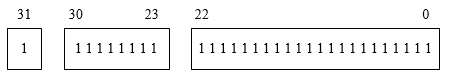
\includegraphics[scale=1]{Binary32.png}
				\end{center}
				\caption{Biểu diễn số thực 32 bits}	
					\label{fig:Bianry32}		
			\end{figure}
		\end{center}			

\subsection*{Bit dấu}
 Bit dấu của số dấu chấm động được biểu diễn bằng một bit. Nếu bit dấu bằng 1 số được biểu diễn là số âm, nếu là 0 số được biểu diễn là số dương. \\
 
 \subsection*{Phần Mantissa}
 	Phần mantissa rất hữu ích cho việc biểu diễn số thực dấu chấm động. Lấy ví dụ $-3.154 \times 10^5$, bit sign là số âm (1), phần mantissa là 3.154 và expoment là 5. Phần thập phân của mantissa là tổng mỗi chữ số nhân với cơ số 10 số mũ của 10 theo vị trí lần lượt từ trái qua phải, đằng sau dấu phẩy:
 	
 		$.154$ = $\frac{1}{10} + \frac{5}{100} + \frac{4}{1000}$
 		
 	Số thực dấu chấm động ở dạng nhị phân rát đơn giản. Ví dụ, trong số $+11.1011 \times 2^3$, bit sign là số dương (0), phần mantissa 11.1011, và expoment là 3. Thần thập phân của mantissa là tổng mỗi chữ số nhân với cơ số 2 số mũ của 2 lần lượt là vị trí của từng chữ số sau dấu phẩy:
 	
 		$.1011 = \frac{1}{2}+ \frac{0}{4} + \frac{1}{16}$
 		
 		Có thể tính phần thập phân của mantissa 1011 bằng cách chia cho $2^4$. Giá trị có được là $11/16 = 0.6875$. Kết hợp với phần nguyên của ví dụ là $11.$ tương ứng là 3, cơ số 10 của ví dụ này là 3.6875. Dưới đây là một số ví dụ khác:
 		\begin{longtable}{|l|l|l|}
 			\hline 
 				Nhị phân dấu chấm động & Cơ số 10 của phần thập phân & Cỏ số 10 \\
 			\hline
 			\hline
 				11.11 & 3 $\frac{3}{4}$ & 3.75\\
 			\hline
 				0.0000000000000000000001 & $\frac{1}{8388608}$ & 0.000001192092895578125 \\
 			\hline
 		\end{longtable}
 		
 		Bảng ~\ref{tb:VDBinary} trình bày một số ví dụ đơn giản cách biểu diễn phần thập phân của số thực dấu chấm động, giá trị cơ số 10 của mỗi giá trị:
 		\begin{longtable}{|l|l|l|}
 			\hline
 				Nhị phân & Phần thập phân & Giá trị cơ số 10 \\
 			\hline
 			\hline
 				.1 & $\frac{1}{2}$ & .5 \\
 			\hline
 				.01 &$ \frac{1}{4}$ & .25 \\
 			\hline
 				.001 & $\frac{1}{8}$ & .125 \\
 			\hline
 				.0001 & $\frac{1}{16}$ &.0625 \\
 			\hline
 				.00001 & $\frac{1}{32}$ & .03125 \\ 			
 			\hline
 			\caption{Ví dụ biểu diễn số dấu chấm động}
 			\label{tb:VDBinary}
 		\end{longtable}
 		
 	 \subsection*{Phần Expoment}
 Phần expoment theo định dạng IEEE short real lưu trữ 8-bit là một số nguyên không dấu có số cơ sở là 127. Lấy lại ví ụ $1.101 \times 2^5$ có expoment là 5, số 5 này được cộng với số cơ sở 127 được tổng là 132 biểu diễn ở dạng nhị phân số nguyên là 10000100. Bảng ~\ref{tb:VDEx} đưa ra một số ví dụ về điều chỉnh phần expoment và được biểu diễn sang số nhị phân:
 	\begin{longtable}{|l|l|l|}
 		\hline
 			Expoment & Điều chỉnh & Số nhị phân \\
 		\hline
 		\hline
 			+10 & 137 & 10001001 \\
 		\hline
 			0 & 127 & 01111111 \\
 		\hline
 			-5 & 122 & 01111010 \\
 		\hline
 			+128 & 255 & 11111111 \\
 		\hline
 			-127 & 0 & 00000000 \\ 		
 		\hline
 			\caption{Ví dụ về expoment}
 			\label{tb:VDEx}
 	\end{longtable}
 	
 	Giá trị expoment sau khi điều chỉnh không được âm. Giá trị nhất của số expoment là 128 khi được công thêm số mũ cơ sở (127) là 255. Đây là số lớn nhất mà 8-bit có thể biểu diễn được. Phạm vi của số mũ trong định dạng short real là $1.0 \times 2^{-127} $tới $1.0 \times 2^{+128}$
\subsection*{Biểu diễn Mantissa về định đạng chuẩn}
	Trước khi số thực dấu chấm động được mã hóa nhị phân lưu chính xác giá trị của số đó, phần mantissa cần phải đưa về dạng chuẩn. Việc xử lý này dựa trên thao tác toán học số thực dấu chấm động. Ví dụ, để biểu diễn số 1234.567 sang dạng chuẩn là 1.234567 $\times 10^3$ bằng cách dịch chuyển dấu phẩy sang trái đồng thời nhân với cơ số 10 số mũ tăng lên theo vị trí mỗi số dịch qua. Số mũ tăng lên khi được dịch qua trái, và giảm xuống khi dịch qua phải.
	
	Tương tự như vậy khi biểu diễn số thực sang số nhị phân. Lấy ví dụ 1101.101 đưa về dạng chuẩn sẽ là 1.101101 $\times 2^3$ bằng cách dịch dấu chấm sang trái ba số đồng thời nhân với  $2^3$. Bảng ~\ref{tb:VDMa} đưa ra một số ví dụ: \\ \\
	
	\begin{longtable}{|l|l|l|}
		\hline
			Giá trị nhị phân & Dạng chuẩn & Số Expoment \\
		\hline
		\hline
			1111.001 & 1.111001 & 3 \\
		\hline
			.0000101 & 1.01 & -5 \\
		\hline
			1.1010 & 1.1010 & 0 \\
		\hline
			100011000.0 & 1.000110000 &  8\\
		\hline
			\caption{Ví dụ biểu diễn số mantissa}
			\label{tb:VDMa}
	\end{longtable}

\subsection*{Biểu diễn nhị phân theo chuẩn IEEE}
	Khi đã biểu diễn được bit sign, phần expoment và phần mantissa theo dạng chuẩn. Biểu diễn các bit theo thứ tự như hình ~\ref{fig:Bianry32}. Ví dụ lấy giá trị nhị phân là 1.101 $\times 2^0$ có bit dấu là 0 (số dương), số mũ hiện là 0 nhưng được điều chỉnh bằng cách cộng với 127 (số cơ sở theo định dạng shorl real)  là 127 biểu diễn ở mã nhị phân là 01111111. Số "1" ở phía bên trái cao nhất của phần mantissa (1.101) được loại bỏ lấy phần sau dấu phẩy là 101. Theo thứ tự bit định dạng  IEEE shorl real là 1 01111111 1010000000000000000000. Bảng ~\ref{tb:VDIEEE} trình bày một số ví dụ:
	\begin{longtable}{|l|l|l|}
	\hline
		Giá trị nhị phân & Expoment & Sign, Expoment, Mantissa\\
	\hline
	\hline
		-1.101 & 127 & 1 01111111 10100000000000000000000 \\
	\hline
		+1101.1110 & 130 & 0 10000010 11100000000000000000000 \\
	\hline
		-0.000101 & 124 & 1 01111100 01000000000000000000000 \\
	\hline
		+1111110001.0 & 136 & 1 10001000 11111100010000000000000 \\
	\hline
		+0.0000001101011& 120 & 1 01111000 10101100000000000000000 \\
	\hline
		\caption{Ví dụ chuản IEEE}
		\label{tb:VDIEEE}
	\end{longtable}	